\chapter{Procesamiento señal de voz}
En este capítulo conoceremos más acerca del procedimiento para procesar la señal de voz, así como también las características para que el lector tenga un mejor entendimiento de esta.

\section{Conceptos previos}
\subsection{Voz}
Los seres humanos diariamente nos comunicamos por medio del habla utilizando nuestras voces somos capaces de transferir información en forma de \textit{ondas sonoras}.\\ Estas ondas transmiten una gran cantidad de información usando el aire como medio de transmisión.
 
\subsection{Audios}
Los audios son un tipo de \textit{datos no estructurados}, es decir datos que no se encuentran en algún tipo de estructura de datos, estos tipos de datos son los que más se encuentran el mundo real como imágenes y audio. Una características de estos es que son complejos en su recolección y preparación para la realización de un análisis.\\ El audio puede capturarse mediante la grabación de nuestro entorno pero para que este audio sea entendido por las computadoras necesita un formato adecuado como: wav, mp3 y wma. \\
Debido a que el sonido es una señal de onda podemos analizar y obtener valores numéricos de este. En la figura 4.1 observamos una onda de la cual obtenemos valores almacenando las alturas de puntos equidistantes de esta forma guardamos información de esta onda.
\begin{figure}[H]
	\centering
	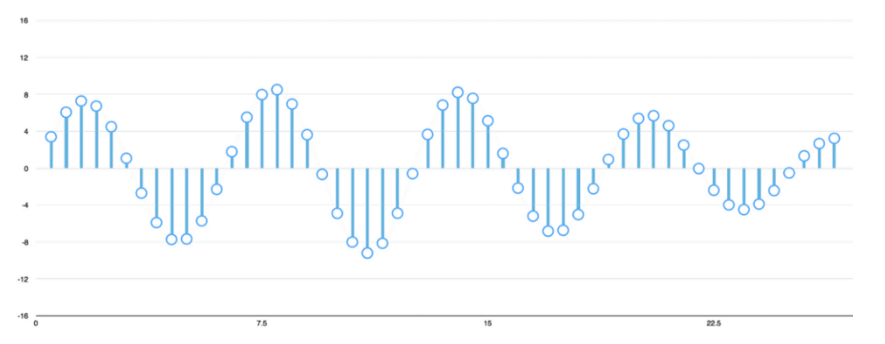
\includegraphics[width=0.9\textwidth]{Figures/onda.png}
	\caption{Onda de sonido \\ Fuente:  \href{https://medium.com/@venkateshpnk22/how-to-convert-your-speech-voice-to-text-data-1b2686099260}{\textit{https://medium.com}}}
	\label{onda}
\end{figure} 
\section{Preprocesamiento}